\section{Roughness propagation}
As described in section \ref{subsec:roughness_prop}, three different test cases were setup to verify the
propagation of the surface roughness values to the proper volume cells.

\paragraph{Cube}
This test was designed to make sure the propagation is sound. Figure
\ref{fig:cube_ks_prop} shows the surface cube with the rough patch in the middle
of each face. The volume mesh is sliced in two axis and the propagation of the
roughness values can be seen.

\begin{figure}[H] \centering
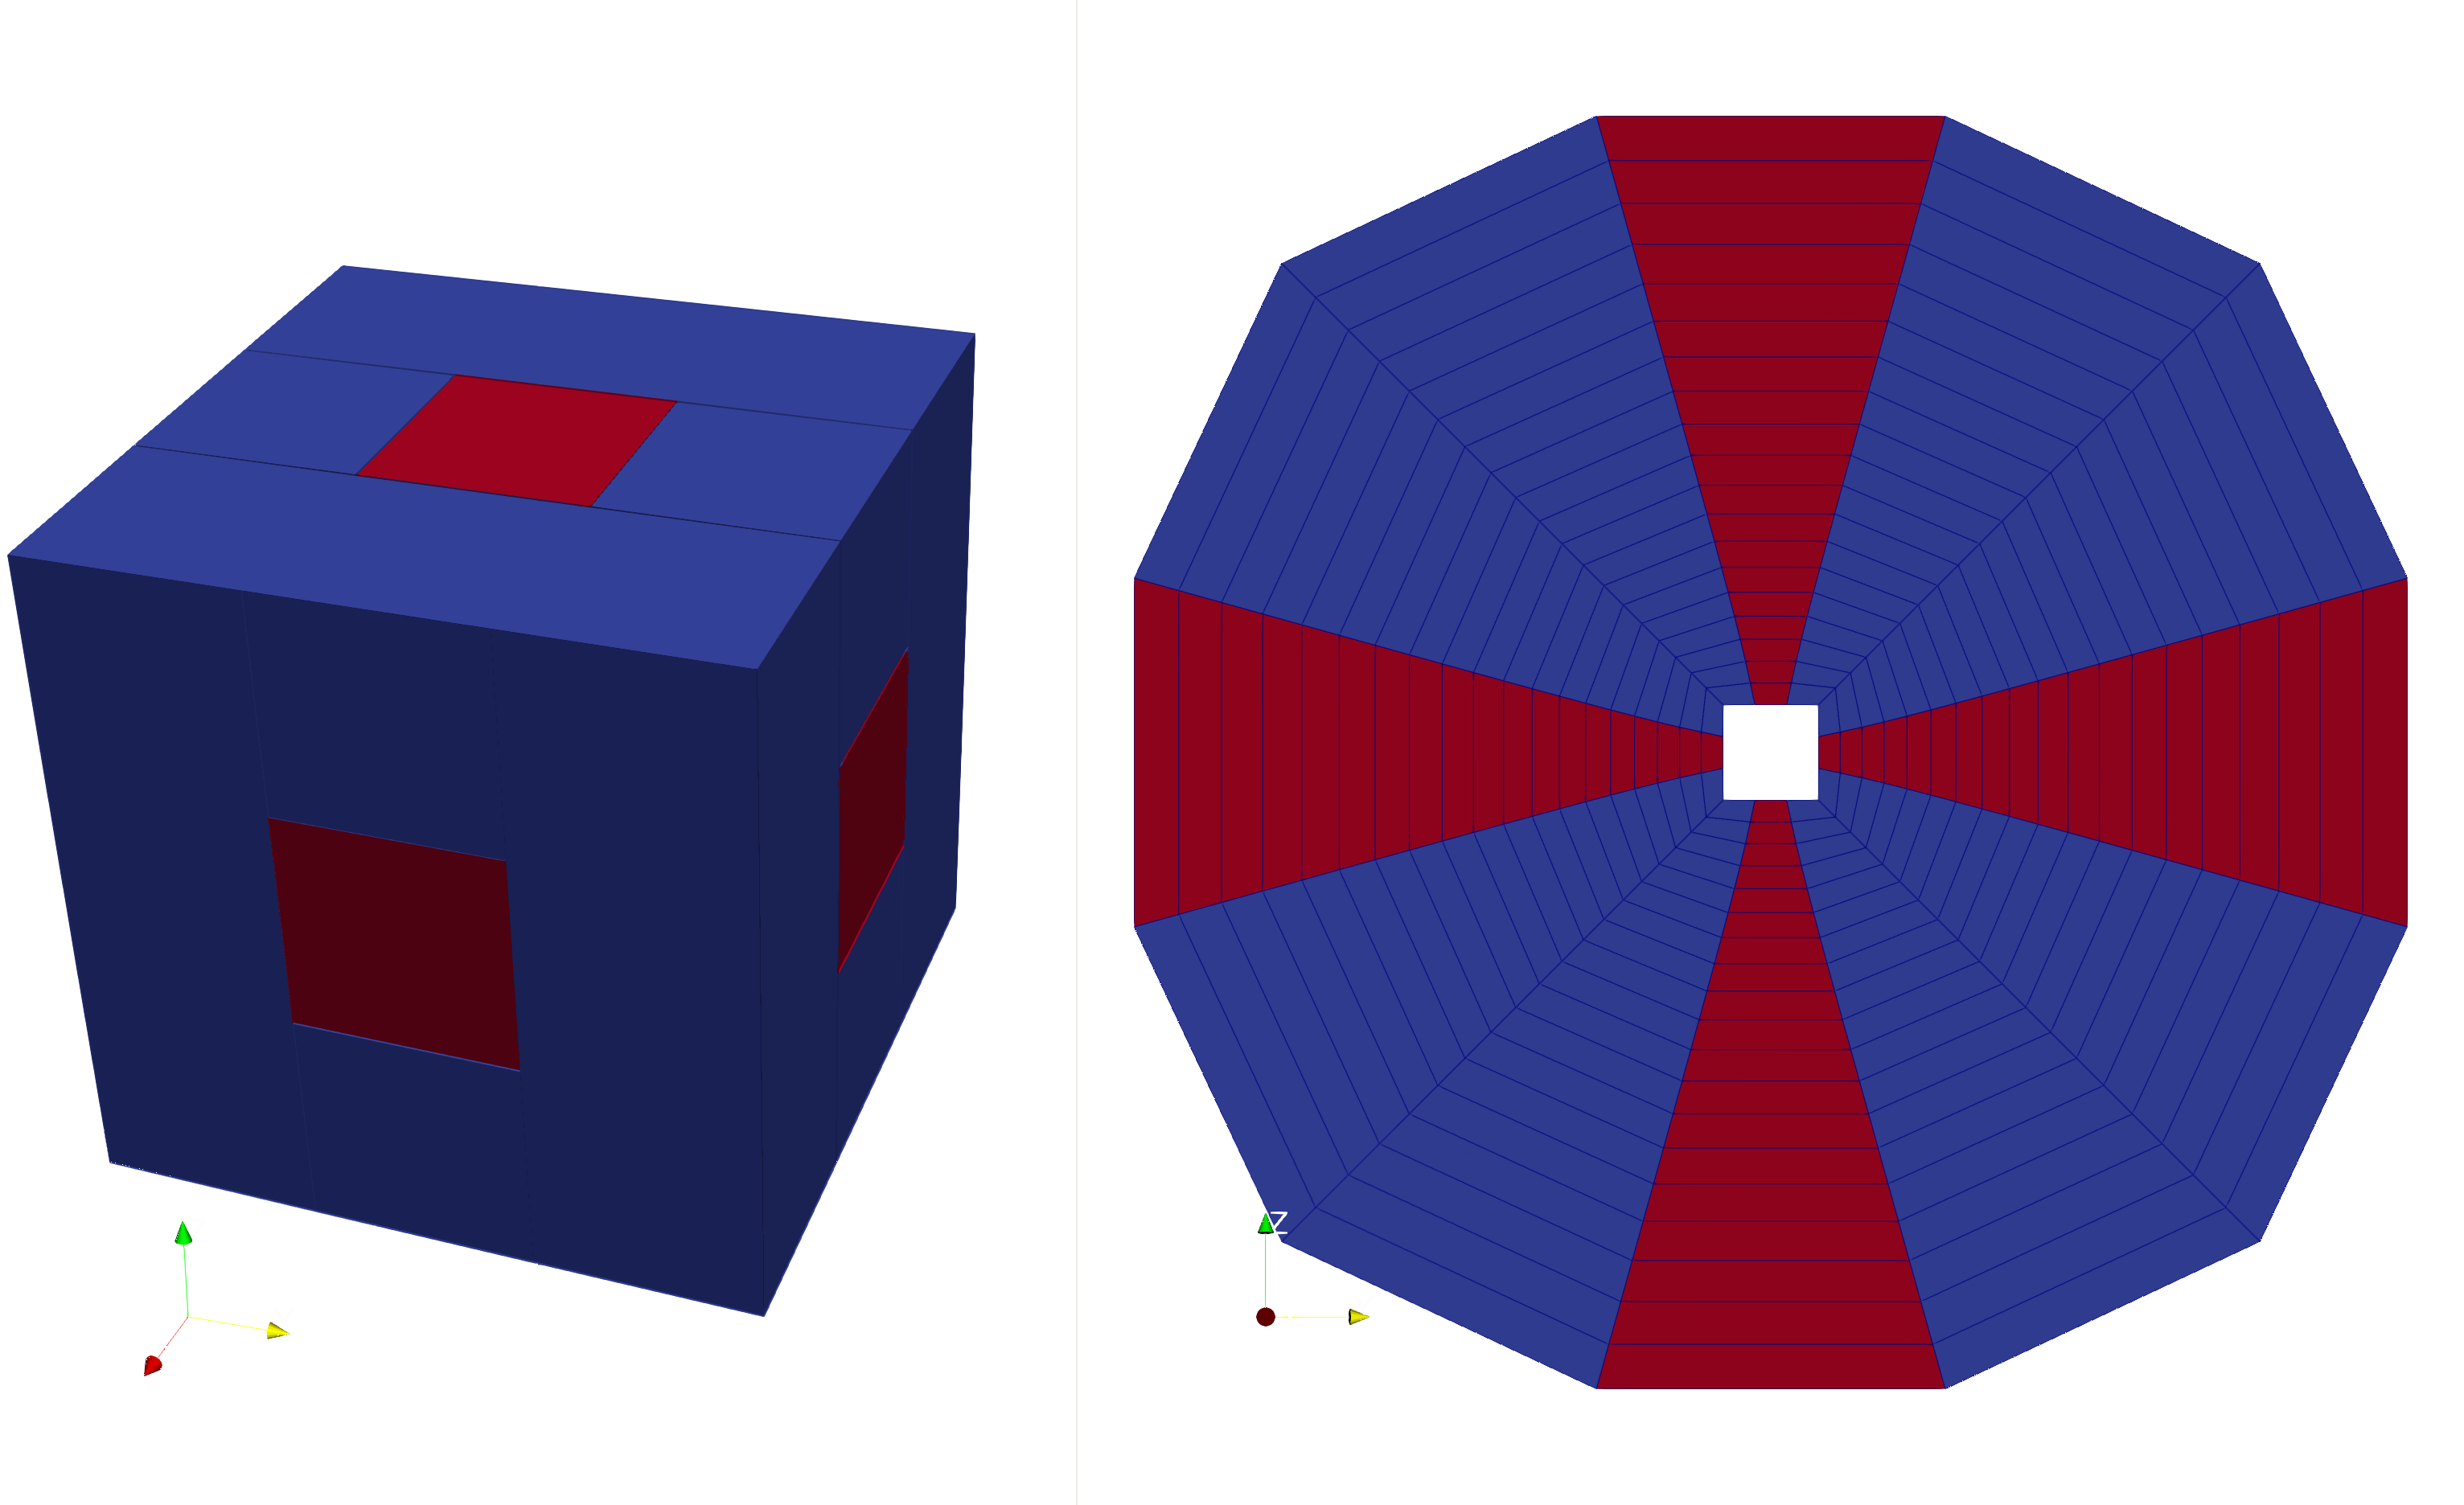
\includegraphics[width=0.7\textwidth]{cube_ks_prop.png}
    \caption{Cube with propagated roughness values. Red equals
$k_{s} = 1.0$ and blue $k_{s} = 0.1$.}
    \label{fig:cube_ks_prop}
\end{figure}

\paragraph{Cuboid}
As described in section \ref{subsec:roughness_prop}, this test case was designed
to catch errors in the correlation of the surface cell to the global cell index
(\texttt{gid}). As such, no figures can be showed. But one can report that all
six cases where each blockface (\texttt{kMin}, \texttt{kMax}, \texttt{jMin},
etc.) was assigned the wall surface, passed with no errors.

\paragraph{Overset cube}
Similar to the previous \texttt{cube} test case, this test shows that the roughness
values are propagated correctly, even when overset meshes are used. As described
in section \ref{subsec:roughness_prop}, it was necessairy to refine the mesh a
bit. This was necessairy as the \textit{implicit hole cutting} would fail
otherwise. In figure \ref{fig:cube_overset_ks_prop}, the two overlapping meshes
are clearly visible.

\begin{figure}[H] \centering
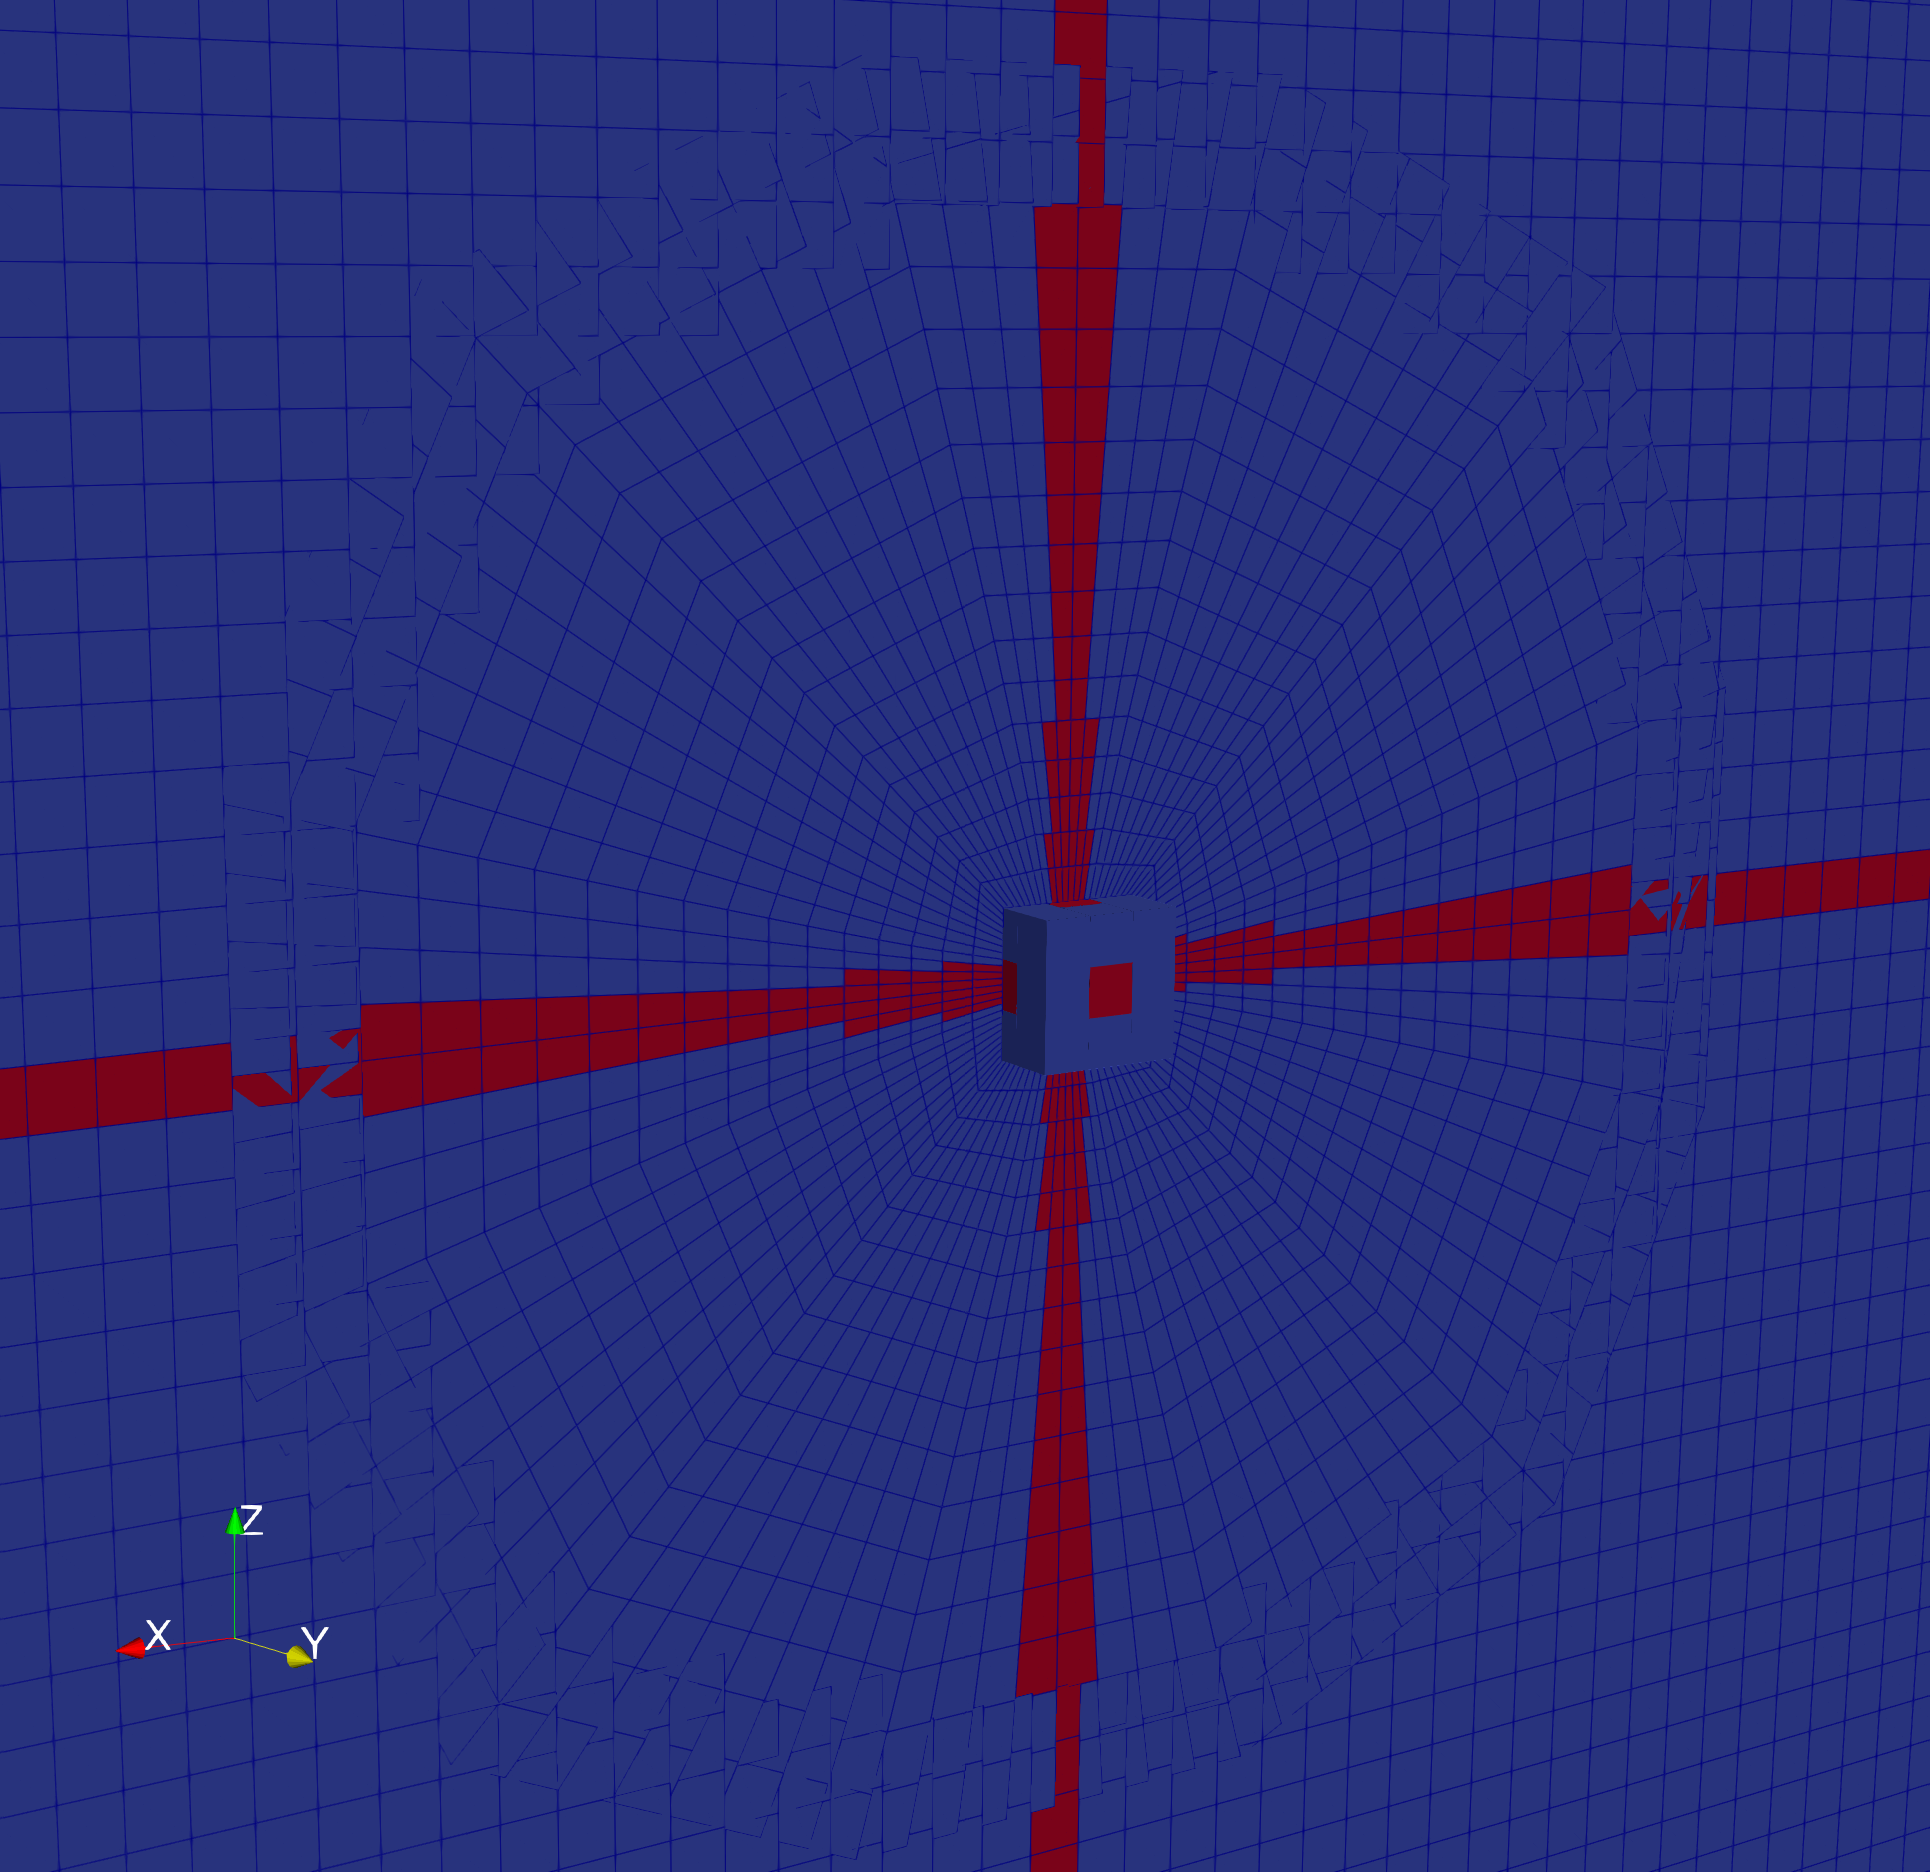
\includegraphics[width=0.7\textwidth]{cube_overset_ks_prop.png}
    \caption{Overset cube with propagated roughness values. Red equals
$k_{s} = 1.0$ and blue $k_{s} = 0.1$.}
    \label{fig:cube_overset_ks_prop}
\end{figure}
